\chapter{
ساخت مدار با
Proteus
}
\section{جمع کننده‌ی Carry-Look-Ahead}
\subsection*{مقدمه و تئوری آزمایش}
برای ساخت جمع‌کننده‌هایی با تعداد بیت‌بالا معمول است که جمع‌کننده‌های کوچک را پشت سر هم می‌بندند.
این کار از جهاتی بسیار مفید است. چرا که به تمیزتر شدن مدار و قطعه‌قطعه یا ماژولار شدن آن کمک می‌کند.
اما مشکلی که این روش دارد این است که هر جمع کننده برای رسیدن به جواب نهایی باید بیت کری ورودی خود را بداند و این عدم آگاهی زنجیروار تا اولین جمع‌کنند می‌رسد به طوری که جمع‌کننده‌ی بیت آخر باید به تعداد تاخیر همه‌ی جمع‌کننده‌های قبلی خود صبر کند تا جواب قطعی درست بدهد.

برای حل این مشکل از قطعه‌ای به نام
\lr{Carry Look-ahead Generator}
استفاده می‌شود که به طور خلاصه این زمان تاخیر را کاهش می‌دهد و کری‌ها را با سرعت بالاتری محاسبه می‌کند و در اختیار جمع‌کننده‌های دیگر می‌گذارد. و در واقع این وابستگی پشت هم قطعات و جمع شدن تاخیر آن‌ها را از بین می‌برد.

\begin{figure}[h]
\centering
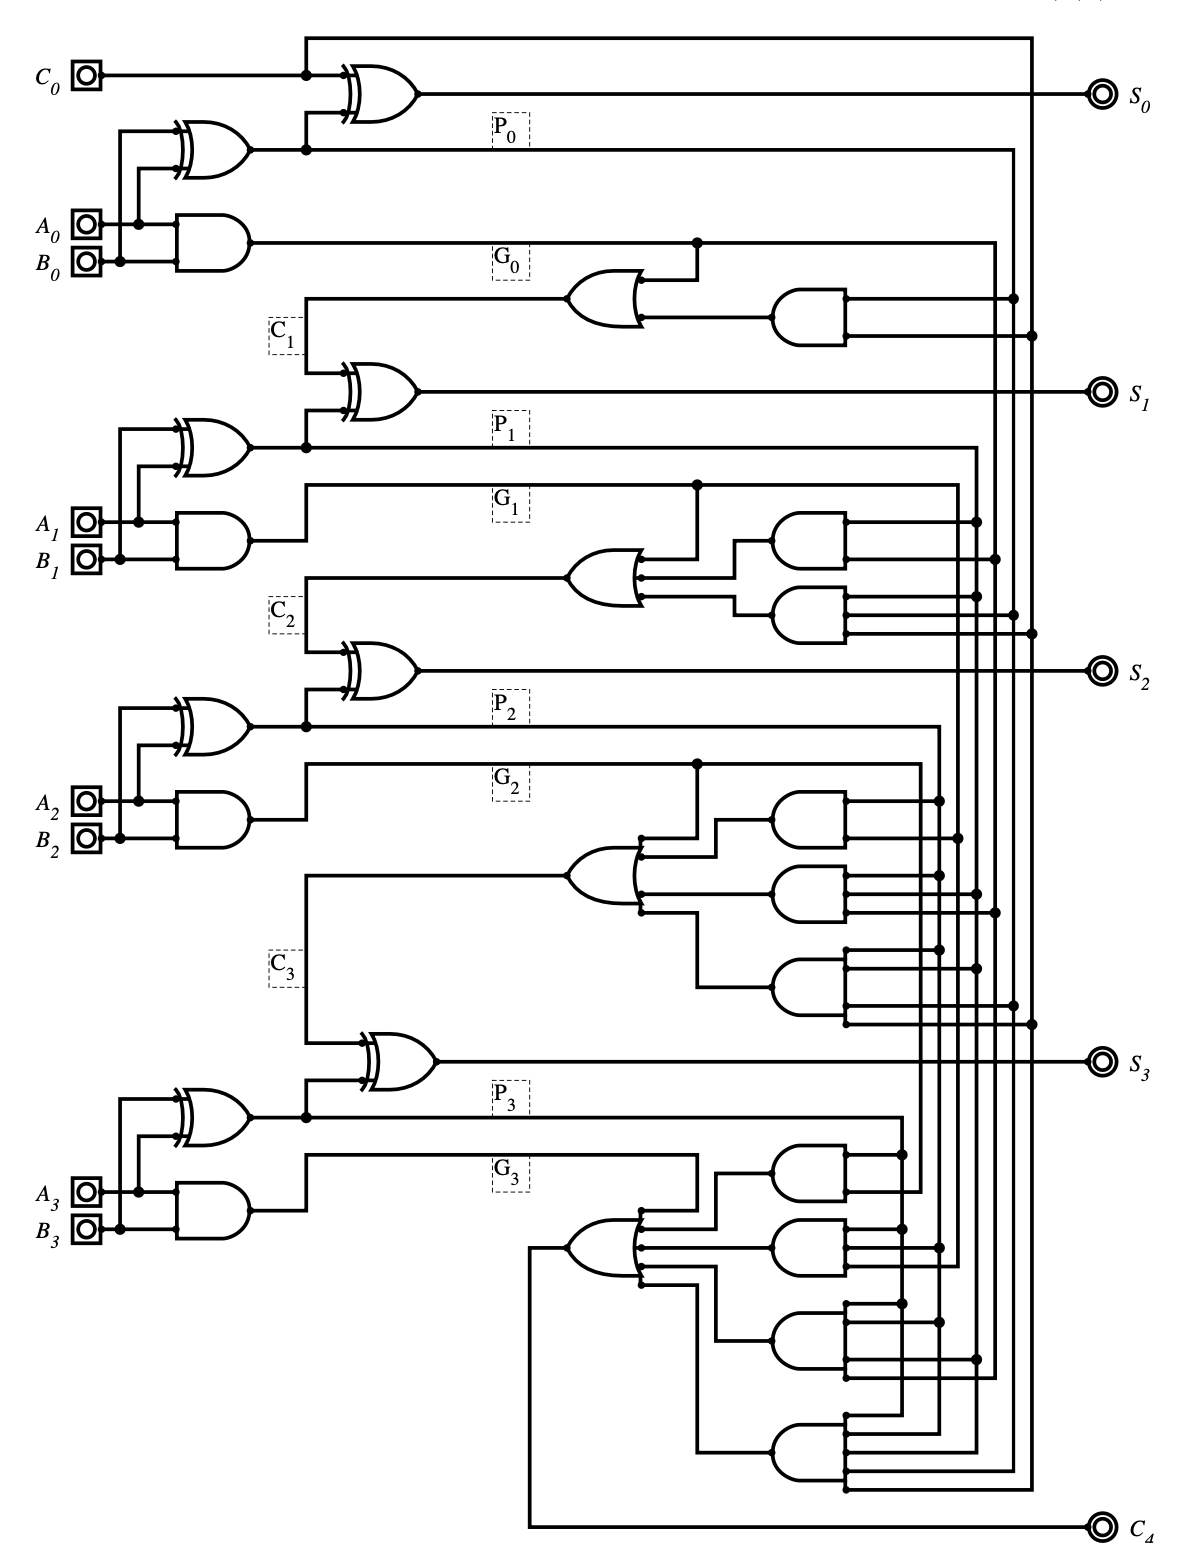
\includegraphics[scale=0.7]{Results/3.png}
\caption{
مدار داخلی یک
جمع کننده 4 بیت با
\lr{Carry Look-ahead Generator}
باز
}
\end{figure}

\subsection*{شرح آزمایش}
\begin{figure}[h]
\centering
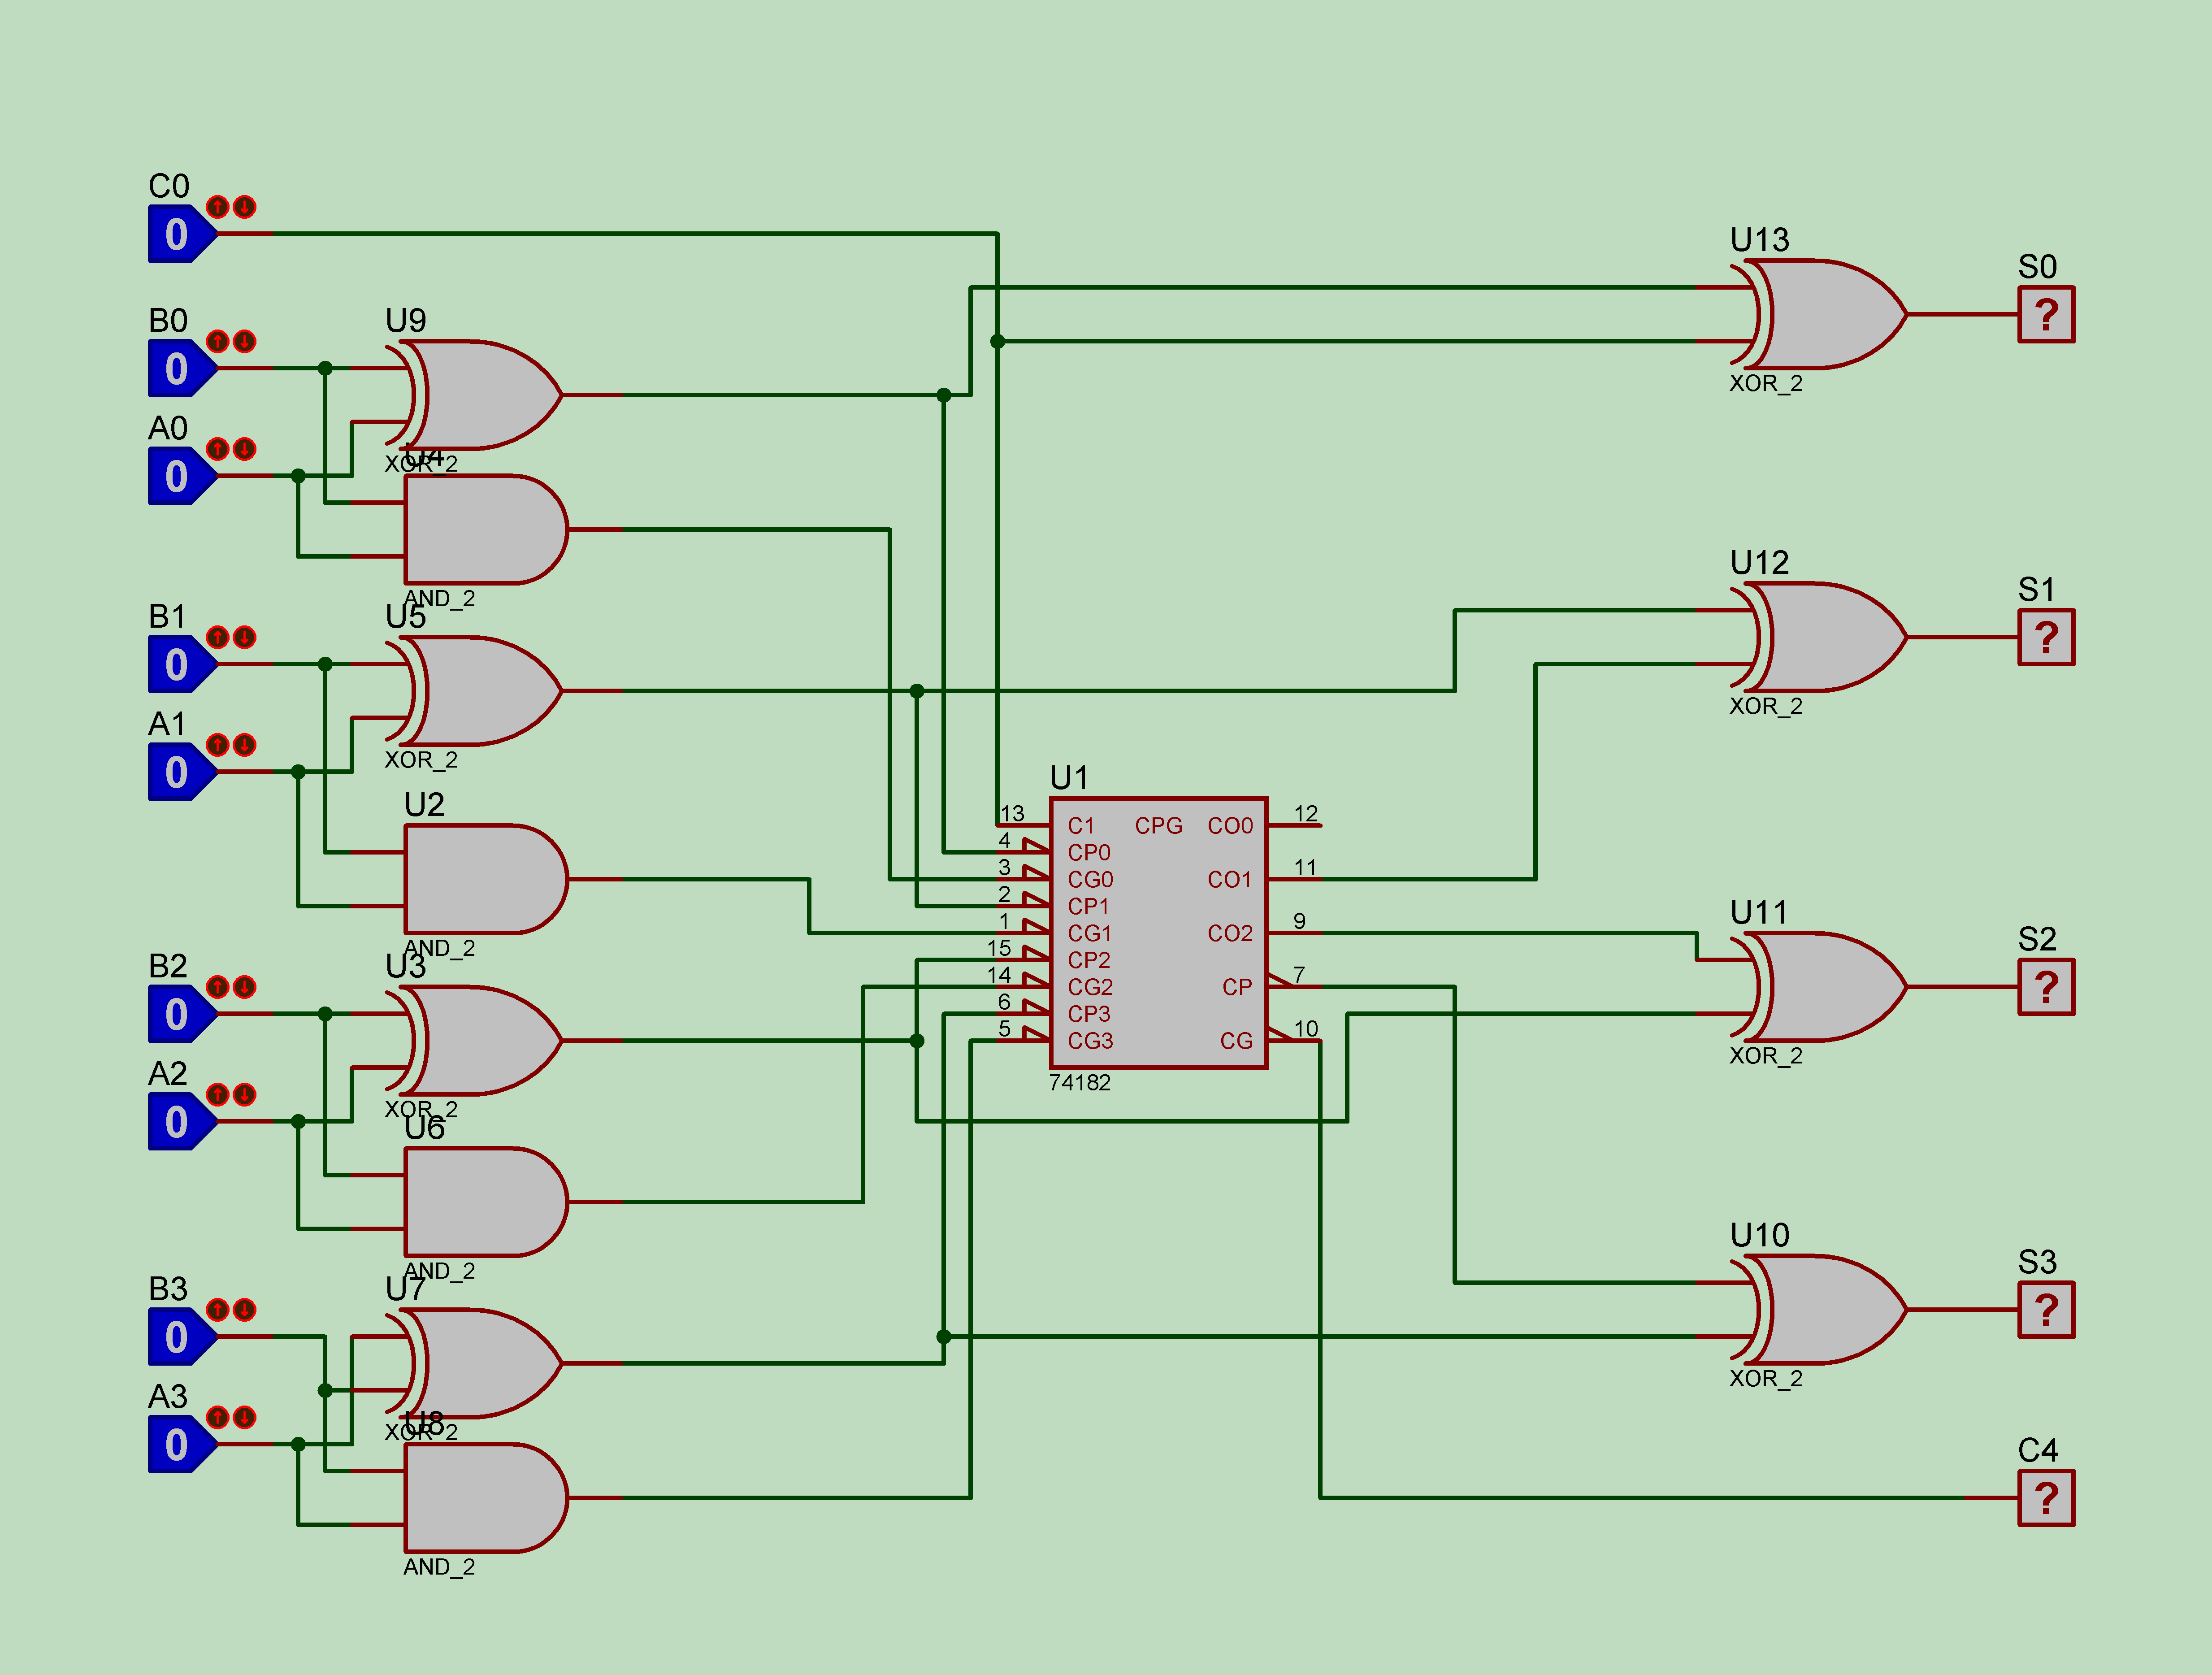
\includegraphics[scale=0.09]{Results/FastAdder.png}
\caption{
جمع کننده‌ی 4 بیتی سریع
}
\end{figure}

مطابق شکل قطعه‌ی 
\lr{Carry Look-ahead Generator}
را از کتابخانه‌ی نرم‌افزار
Proteus
پیدا کرده و قرار می‌دهیم سپس مطابق تئوری گیت‌ها و ورودی‌ها و خروجی‌ها را وصل می‌کنیم و برای آن‌ها نام می‌گذاریم.

